% IMPORTANT! In order for the document to compile, one needs to use XeLaTeX or LuaLaTeX as compiler. This can be done in  Overleaf by Menu -> Settings -> Compiler -> Choose XeLaTeX/LuaLaTeX
\documentclass[t,24pt,aspectratio=169]{beamer}

\usepackage{KUstyle}

\toplinje{TMU} % The text at top. Remove the command if no text is desired

%\documentclass[aspectratio=169]{beamer}
\title{Holistic OMS 全人口腔顎面外科}
\date[today]{\today}
\author[Name]{祁力行}
\institute[Oral and Maxillofacial Surgery]{Wan Fang Hospital, Taipei Medical University, Taipei 116, Taiwan}
%\usetheme{lumc}% theme

\setbeamertemplate{frame numbering}{%
  \ifnum\insertframeendpage>\insertframestartpage{}
        \insertframenumber{} -- \insertoverlaynumber{}%
  \else
        \insertframenumber{}
  \fi%
}
\makeatother



%\beamertemplatenavigationsymbolsempty

%\setbeamerfont{page number in head/foot}{size=\large}
%\setbeamertemplate{footline}{\insertframenumber/\inserttotalframenumber}
%{
%  \leavevmode%
%  \hbox{%
%  \begin{beamercolorbox}[wd=.333333\paperwidth,ht=2.25ex,dp=1ex,center]{author in head/foot}%
%    \usebeamerfont{author in head/foot}\insertsection
%  \end{beamercolorbox}%
%  \begin{beamercolorbox}[wd=.333333\paperwidth,ht=2.25ex,dp=1ex,center]{title in head/foot}%
%    \usebeamerfont{title in head/foot}\insertsubsection
%  \end{beamercolorbox}%
%  \begin{beamercolorbox}[wd=.333333\paperwidth,ht=2.25ex,dp=1ex,right]%{date in head/foot}%
%    \usebeamerfont{date in head/foot}\today \hspace*{2em} % insertshortdate{}
%   \insertframenumber / \inserttotalframenumber\hspace*{2ex} 
% \end{beamercolorbox}
% }%
%  \vskip0pt%
%}

%\usebeamerfont{footline} 
%   \insertframenumber/\inserttotalframenumber
%\usepackage{ifthen} % for If with condition: \ifthenelse{condition}{A}{B}

\usepackage{adjustbox} % for minipage to the right

\usepackage{tabularx} % for resizebox?

%\usepackage{CJKutf8} % by pdfLaTeX, not LuaLaTeX
% *** https://www.math.sinica.edu.tw/www/tex/default14.jsp
\usepackage{xeCJK} % for Chinese, compiling by XeLaTex

\usepackage{fontspec} %設定字體
% Fandol font (the default)  not shown "內"
\setCJKmainfont{AR PL UMing TW MBE} % AR PL UMing TW MBE or "UKai" https://www.overleaf.com/learn/latex/Questions/Which_OTF_or_TTF_fonts_are_supported_via_fontspec%3F#Chinese
%BiauKai} %標楷體 from macOS %設定中文為系統上的字型,而英文不去更動,使用原TeX字型

\XeTeXlinebreaklocale "zh"
\XeTeXlinebreakskip = 0pt plus 1pt %這兩行一定要加,中文才能自動換行

\usepackage{outlines}



\begin{document}

% The first slide. One can for instance change the main title, the subtitle, speaker, KU-unit and date
{
\setbeamertemplate{background}{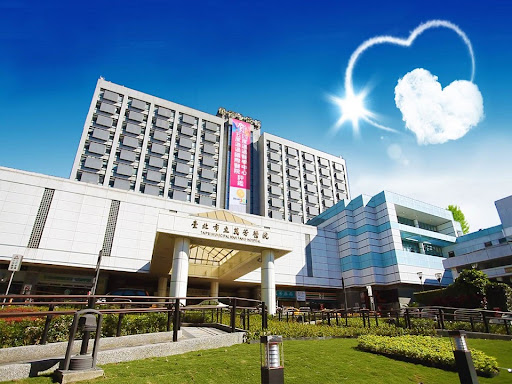
\includegraphics[width=\paperwidth,height=\paperheight]{KU/TMWH_front.jpg}} % forside.pdf
\begin{frame}
    \begin{textblock*}{\textwidth}(0\textwidth,0.1\textheight)
        \begin{beamercolorbox}[wd=7.8cm,ht=7.3cm,sep=0.5cm]{hvidbox}
            \fontsize{5}{10}\fontfamily{ptm}\selectfont \textls[200]{Wan Fang Hospital, TMU}
            \noindent\textcolor{KUrod}{\rule{6.8cm}{0.4pt}}
        \end{beamercolorbox}
        
\includegraphics[width=1cm]{KU/TMWH_logo.png}
    \end{textblock*}
    \begin{textblock*}{\textwidth}(0\textwidth,0.1\textheight)
        \begin{beamercolorbox}[wd=7.8cm,sep=0.5cm]{hvidbox}
                \Huge \textcolor{KUrod}{Holistic OMS 全人口腔顎面外科}
                \vspace{0.5cm}
                \par
                \Large 萬芳口外的現況與未來
                \vspace{0.5cm}
                \par
                \normalsize Speaker, 祁力行, \today
        \end{beamercolorbox}
    \end{textblock*}
    \begin{textblock}{1}(7.7,13.38) %8.3,11.38
        
\includegraphics[width=8cm]{KU/TMWH_logo.png}
    \end{textblock}
\end{frame}
}

% A standard slide. It's important that [hoved] is included after \begin{frame}
\begin{frame}[hoved]
\frametitle{心得}
2021/04/01 科主任到任以來,一直記得的初衷
\begin{outline}
\1 櫻翠的專科考試及SCI paper
\1 以華的專科訓練及考試、查房教學
\1 柏仁的專科訓練
\end{outline}
因為萬芳口外的處境,讓大家替三位優秀的住院醫師擔心。\\
如此,四個月過去,祁力行很傷心,因為二位住院醫師即將離職。我們沒有能力留下他們,因為萬芳口外生病了。

以內部審查委員的角色,檢視這四個月的發現,科主任以為,問題的核心是萬芳口外只有人治,沒有制度。因此不夠細心,即使2020已經發現專科考試3.5的年資,「PGY1必修不計」,仍以交情好人脈廣為理由,讓孫醫師以為報名資格不會有問題。也因為人脈廣,甚至讓唐醫師的專科考試有著變數。學弟柏仁看在眼中,原本尚在考量的口外與家庭的選擇,終於也浮現了明顯的答案---家庭。
\end{frame}



\begin{frame}[hoved]
\frametitle{心得}
科主任知道,在於院長室的高度,能夠看到的僅有數字與績效,這是部主任沈重且甜蜜的負擔。對於一個已經病重的萬芳口外,科的存活、維持照顧病患的存活、維持急診值班病房門診的基本安全運作,已然非常吃力。
\begin{outline}

\1 2021/06之前的開刀房業績(每月,含特材)大約60--70萬元
    \2 手術室認養使用率 130\%, 正顎手術收費 20--40 萬元

\1 門診業績(五位 VS,每月) 2021 (一月至三月): 
    \2 專任VS 160--250萬元(mean=200) , total (加上兼任) 240--370 (mean=300); 68\% 為專任VS業續
    \2 專任VS 平均月業績(健保+自費),周最高(77--120萬元, mean 97),冠楊侯 (20--60 萬元),方 (浮動); 
    \2 周門診業績,佔全體 40\% above,若是周加上楊則超過 50\%
    \2 冠州穩定沒有變化,侯殿後
\1 整體趨勢很穩定。2020一整年亦是如此。
\end{outline}
科主任以為,在VS多於fixed R + PGY 的情況,萬芳口外的業績達到瓶頸。
\end{frame}

\begin{frame}[hoved]
\frametitle{口外訓練機構填表 109 (2020) 年度手術統計}

\begin{outline}

\1 [開刀房] 人數
    \2 附醫 134(468)(阻生齒 134);口腔癌42,正顎 25,TMD 9。 
    \2 萬芳 129(362)(阻生齒  42);口腔癌27,正顎 22,TMD 26。

\1 [門診] 顆數 
    \2 附醫 拔牙4363;阻生齒1340;人工植牙 810 。
    \2 萬芳 拔牙3053;阻生齒656;人工植牙 96。
    
\1 []
\1 小結: 人數差異不大,萬芳口外牙齒顆數顯著較少,人工植牙少,而TMJ disorder 手術很多。
\end{outline}
\end{frame}

\begin{frame}[hoved]
\frametitle{心得}
比較驚奇的是,四月份當科主任開會中提到業績不好時,眾位VS的反應是立即而且不服氣的,他們想要知道的是口外與整個牙科部的比例。四個月過後,的確觀察到VS們是樂意看診、安排開刀房手術,急診收治骨折病患PCR陰性後立即開刀。在五、六月間疫情緊繃時,仍然顧著口腔癌病患的急迫,不管分流分艙堅持收治進開刀房手術,在頭頸癌會議中獨排眾議,堅持治療的方式。但專科護理師也因為不願意冒險被帶進開刀房跟刀,第一個選擇離職的路。


科主任以為,醫師費PPF 0.55--0.6 的比例,不止超過北醫附醫牙科(up to 0.3),更是超過一般牙科科所(0.5),是不是也許就是VS努力的目標。曾經看到 intern交接本上,寫著「某某VS動作很快,要跟上」,「某某VS的指令是多做事、少問問題」。VS不敢放刀給總醫師,以華、櫻翠多年來很少有主刀major surgery的機會。理由可能是「因為她們的做法不是我們教的」,而更重要的理由是「病患刀數排得多,VS自已開刀比較快」。
在推行全人醫學教育的科主任心中,這是很令人傷心的事。
\end{frame}



\begin{frame}[hoved]
\frametitle{心得}
傷心的科主任,也多次詢問自己,為什麼還要在萬芳口外繼續上班。因為有著部主任的支持,北醫附醫師長同仁的打氣,更重要的是唐醫師的堅持與勇氣,孫醫師也將總醫師的責任交託給科主任。科主任帶著 booking reading (for intern PGY),門診教學、急診值班指導,全人照顧醫學的使命,是科主任在萬芳口外努力的動機。科主任相信,在跌倒谷底的時候,正是轉型的唯一契機,由附醫口外引進從未存在的萬芳口外制度,要讓VS投資萬芳口外(改變薪質結構)、重拾教學的信心與熱誠。然後,直接受惠的是病患,反應出來的就會是院長信箱的感謝,以及業績指標。
\end{frame}



\begin{frame}[hoved]
\frametitle{方致元醫師的任務}
\begin{outline}
\1 屬意 OGG 與 人工植牙,業績起伏不一定
\1 帶動研究,媒合基礎研究老師與臨床醫師
\1 每週門診數2 (專V 規定6-8診,可含刀日),所以宜增加二至三診
    \2 2021/07/31 科務會議中,科主任邀請方醫師加診,婉拒。
\1 2021/04/07 自費two-jaw OGS手術僅收半價十萬元,sythesis 耗材30,000元。扣除特材後,PPF 7萬元 $x 0.6 = 42,000$左右。
    \2 「致元,這個手術如此辛苦,不是應該可以收 20萬元嗎?」
    \2 致元回答: 「患者是矯正科學妹,培養長期人脈,希望以後能轉診來萬芳」
\1 小結: 科主任不會帶人,不會管理人。而萬芳口外的老闆們其實是各位VS們。
\end{outline}
%致元只靠OGG or 人工植牙(他專攻此項而已)。
%任務編組,致元的職掌是負責研究事宜 (只是延續),其他V 負責其它。現在有得力負責的教研秘書大力協助,其負擔並不重,實不宜當作業績不夠的藉口,大可增加其門診數 (專V 規定6-8診,可含刀日),而不只是專攻植牙、OGS... 真要專攻,也得闖出名號或效率,都排滿而被驗收得到相當的業績才是... 

%orthognathic surgery, two-jaw surgery
%2021/04/07 自費手術十萬元,sythesis 耗材30,000元。
%所以扣除特材後,7萬元x0.6=42,000左右。
%「致元,這個手術如此辛苦,不是應該可以收 20萬元嗎?」

\end{frame}

%\begin{frame}[hoved]
%\frametitle{OR}
%經門診收治住院:(二級警戒中)
%萬芳醫院目前(\today)「限收治癌症或有醫療急迫性病人為原則」


%\end{frame}

\begin{frame}[hoved]
\frametitle{回答}
活在自己的世界裡,而且過於自信和樂觀

\begin{outline}
\1 以全人教育的理想,對人的善良與同理心、慈悲心很樂觀
\1 完全沒有自信,在萬芳口外的小世界裡,其實只是為了一心照顧 intern PGY 及唐醫師,完全沒有管理員工的信心
\1 要多向部主任和彭主任學習
\end{outline}

\end{frame}

\begin{frame}[hoved]
\frametitle{回答}
很少來找部主任商議前因後果,是完全驗收最後成果嗎?
萬一是不可收拾的結果呢?
\begin{outline}
\1 科主任一方面在檢點萬芳口外,一方面在收拾驚訝、傷心
\1 收拾殘局中,人力缺口,要一一克服急診值班問題,了解計劃離職者,對萬芳口外的建言
\1 最壞也是最好的結果,如同彭主任的推測,若VS全部離職。那麼,也就是制度重新建立的開始。
\end{outline}

\end{frame}

\begin{frame}[hoved]
\frametitle{回答}
口外科內的負面聲量已出來,他的過於不以業績為導向的理念和宣
示,已由科內外傳出,這種culture shock過激(2021/07/31 週六晚上的口外科務會議) 
\begin{outline}
\1 科主任的想法,沒有事先報告部主任,對不起,謝謝部主任給予說明的機會
\1 科主任沒有在考量VS的稱讚,只想收拾殘局,保護病患,目前只能醫療業務只能量力而為
\1 「不以業績為導向」的說法
    \2 是事實,因為沒有 fixed R,PGY 的工時、值班,都在重重規範之中,只剩下VS獨立運作,只能先要求安全、站穩腳步先,這是科主任必須優先考量的重點
    \2 是策酪,一句話能反應出VS的心情,所以VS們真的很在乎業績,PPF,科主任要想辦法建立適合萬芳口外的制度,才能讓VS在此安心立命

\end{outline}

\end{frame}

\begin{frame}[hoved]
\frametitle{回答}
櫃檯甚至報告他的週六診大遲到、沒出現
\begin{outline}
\1 每週六 07:30-08:30 am,林永和老師主持 口外口病討論會,數年來祁力行都是指導老師之一,一定出席
    \2 這個診次是VS們一開始替科主任安排的,理由是「(周三與周六上午)因為其他時段 PGY intern 不足」
    \2 接下來有必須做調整,對不起造成櫃臺作業的困擾

\end{outline}


\end{frame}


\begin{frame}[hoved]
\frametitle{回答}
櫃檯甚至報告他拒看不喜歡看的患者(掛他的診)
\begin{outline}
\1  櫃臺指出的「拒看不喜歡看」
    \2 其實力行不明白,可以猜測的是,也許有幾次,PGY intern 回報「指名要製作咬合板」「調整咬合板」
    \2 力行實話實說「我不會做,也不曾做過,要不要請專長的醫師來處理」,周珊如醫師 應該是專家。
\1 櫃臺、門診助理、PGY intern 都曾問過力行「主任您花費了二個小時,詢問、講解,解決睡眠 關節 討論智齒神經,可是都沒有辦法申報,這要如何賺錢」
    \2 患者有緣份,來到力行的門診,看見的不止是他的人,還有他的心與一旁的家人。
    \2 花費這個時間,力行心裡認為很值得
    \2 讓患者找到,幫助自己癒合的最好方式,而且試著預防下一次的問題
    \2 頂多是申報 TMJ F920270c 1000點,或者是雷射針灸 400元。
    \2 萬芳醫院經門診收治住院:(二級警戒中)目前(\today)仍「限收治癌症或有醫療急迫性病人為原則」,也只能讓擁有深部智齒的患者,暫時先等候。
\end{outline}


\end{frame}


\begin{frame}[hoved]
\frametitle{回答}
業績是萬芳的基本盤,就算自己的style做不到,也要有能力讓科業績做起來,更何況自己的業績和科內主力型V差太多,何以服眾?難道他的教學和研究能超級突出?
沒有臨床cases何富務實的臨床教學?

\begin{outline}
\1 萬芳口外的業績,來自重建制度,VS才能安身立命,重新發揮服務,然後兼顧教學研究。
    \2 目前除了方醫師,VS覺得門診開刀房的服務已經很吃緊
    \2 科主任發現前述綜論的問題,以為正是萬芳口外業績的瓶頸,要讓業績增加,努力的點也在此
    \2 科主任在學習當科主任,以為培育營造優質的土壤,才能是口外發展的根基,讓VS有舞臺展現業績、教學及研究。

\end{outline}

\end{frame}

\begin{frame}[hoved]
\frametitle{評分萬芳口外業績}
\begin{outline}
\1 以下的觀察加入力行個人的評論,僅供參考
    \2 萬芳口外 2020-2021/04 既有的業續量,不知該用什麼基準點來評分
    \2 醫療業務的質,不可思議
        \3 門診業續量大,MRI 量大,容易被健保抽查檢視
        \3 全身麻醉手術案例,在口外學會討論會、三院口外口病討論會,報告的案例,手術品質、自費骨粉耗材的使用時機,有諸多可以討論的空間
        \3 林冠洲醫師的二位口腔癌病患,執行非主流且不是NCCN 指引規範的「光動力療法」,並非申請人體臨床實驗計劃,而是衛福部恩慈療法的專案進口藥物(光療藥物),有違萬芳頭頸癌團隊的建議治療方案。亦造成「計畫書符合診療指引 」指標項目的扣分案例。其中一位患者,目前因照光部位(腫瘤)上顎骨壞死入院手術,病理報告(待)應該會發現口腔癌細胞。
%        \3 醫者在臨床工作上本該為病人在各種不同的治療方式中,選取成功率較高的治療方式、以病人之利益為依歸,包括將沒有把握的案例轉介給適當的同業,或是自己實際操作教學予PGY intern,都是行善原則的表現。
        \3 VS們對於科主任查房,持有不同的意見,進而阻止科主任隨同總醫師查房。平日各主治醫師查房均不定時,總醫師無法分身隨同(忙於開刀房、門診),而由專科護理師隨同、轉達,此舉對於醫學教育的傳承,恐有不周全。(2021/04/27 向施副院長報告)。
    
\end{outline}


\end{frame}

\begin{frame}[hoved]
\frametitle{口外開刀房的問題}
手術室耗材採購的方式: 發票給牙科秘書、器材直送刀房淑妃

\hl{
沒有建立醫院的耗材碼 (ex: 各種bur的型號),手術的工具就沒有醫院的保障與背書。
}



\begin{outline}
\1 林冠州醫師 :拿廠商的發票來先向牙科部核報,而器械先寄放在廠商處,未來需要時再請廠商送貨。經查閱發票有三張:
\2 2020/05/04 鏵品 65,400元 (已於 2020/08/17 全數交貨完畢)

\2 2020/07 威司美 Stryker 78,300 + 31,100 元
    \3 交貨情況待查
    \3 2021 經銷商已換為博新

\1 三張發票小計為 174,800元

\end{outline}



\end{frame}



\begin{frame}[hoved]
\frametitle{Todo list:}
\begin{outline}
\1 <人員配置>(專任VS 六名) - Fix R: 0 人,資深「外交」部總醫師 1 - PGY: 2人
 - Intern: 4人
\1 維持口外訓練機構
\2 建立:手術、病理切片統計 database
\2 修訂:口外住院醫師訓練計劃書(更新為3.5年)
\2 聯合三院辦理專科考試訓練班(幫助以華、櫻翠)
    \3 櫻翠的 manuscript 即將完成,投稿在即
    \3 櫻翠研究所開學,GP門診略減(更名為口腔顎面外科門診),祁力行增加診次(取代部分櫻翠在GP 的時段及診間)
    \3 櫻翠 幫忙照顧祁力行、周珊如醫師的手術、住院病患。至專科醫師考試完成。
\1 維持 PGY intern 教學 meeting
\2 Intern 第一線值班(每週4--5日),具領值班費,由科主任、VS、資深住院醫師第一線指導



\end{outline}
\end{frame}

\begin{frame}[hoved]
\frametitle{長期規劃}
\begin{outline}
\1 修訂:口外VS PPF 要調降為 0.2--0.3 每月浮動(由部主任依照牙科部整體營運來調整),VS support 牙科部教學與經營,而不被高額PPF 吸引全部的注意力。

\1 徵召 fixed R 時機
    \2 口外重建後
%就是要跌倒谷底,才有辦法改革改造;合則聚,不合則散。

\1 維持三院口外口病的討論會,培養共識、增強口腔病理診斷照護的實力

\1 癌症病人治療,邀請附醫口外團隊報備支援,克服手術時技術問題,最终目標在萬芳醫院訓練切除及重建的口腔癌照顧團隊
\end{outline}

\end{frame}


%\begin{frame}[hoved]
%\frametitle{Suggestion and Treatment Plan}

%\end{frame}








\end{document}